\section{Application to CMB maps and power spectra estimations}
\label{sec:cmb}
The measurement of CMB polarization, and especially the detection of $B$ modes, is one of the major challenges in modern cosmology. In this section, we show that the KIDs systematic effect such as the non-linearity does not affect them from detecting $B$ modes.\\

A measure done by a KID is defined by Eq.~(\ref{eq:eq-NL}):
\begin{equation}
m  \simeq (I + \varepsilon I^{2}) + (Q + 2\varepsilon IQ) \cos(2\alpha) + (U + 2 \varepsilon IU) \sin(2\alpha),
\label{eq:eq-NL}
\end{equation}

with \eps\ the non-linearity coefficient.

The non-linearity coefficient depends on the detector response. In fact, it is a systematic effect of the instrument and as a consequence will always impact our measurements. This non-linearity can lead to leakage of the CMB and dust temperature signal into the polarization maps and consequently can induce spurious polarization signals which could prevent us from detecting $B$ mode polarization. \eps\ is constituted of several components such as \eps\ related to the CMB and dust. $T_{dust}$ has more effect on the leakage than $T_{CMB}$  that is why we will focus on dust.
To study this effect we simulate spurious signals from a map of the galaxy (dust) observed by Planck (REF) by applying the non-linear mapping described by Eq.~(\ref{eq:eq-NL}) :

\begin{eqnarray}
\label{eq:spurious-mapI}
\Delta I_{dust}  &=& \varepsilon I_{dust}^{2},\\
\label{eq:spurious-mapQ}
\Delta Q_{dust}  &=& 2\varepsilon I_{dust}Q_{dust},\\
\label{eq:spurious-mapU}
\Delta U_{dust} &=& 2 \varepsilon I_{dust}U_{dust}.
\end{eqnarray}

To investigate the different modes of CMB polarization we used the HEALPix package \citep{2005ApJ...622..759G} to generate modified power spectra from the spurious polarization maps. They are described by Eq.~(\ref{eq:eq-cl}) and are represented in Fig.~\ref{fig:cl2}.

\begin{equation}
\Delta C_{l} = \varepsilon'^{2} C_{l}^{XX'},
\label{eq:eq-cl}
\end{equation}
Where $\lbrace X,X' \rbrace$ = $\lbrace T,E,B \rbrace$ .\\

\begin{figure}[h]
\center
	\includegraphics[scale=0.5]{Figures/cl2_spurious.eps}
	\caption{Power spectra for spurious temperature and polarization anisotropies. The black, blue and red curves indicate the $EE$, $TE$ and $BB$ power spectra. The bottom three red curves represents the $BB$ power spectra for a tensor-to-scalar ratio r = (T/S) = 0.1, 0.01, 0.001.}
	\label{fig:cl2}
\end{figure}

Here we will focus on the leading spurious term $C_{l}^{TE}$ : 
\begin{equation}
\Delta C_{l}^{BB} = \varepsilon^{2} C_{l}^{TE}.
\label{eq:eq-cl2}
\end{equation}

The leakage of temperature into polarization is represented by the coefficient \eps\ of Eq.~(\ref{eq:eq-cl2}). To determine this coefficient, we compute :

\begin{equation}
\varepsilon = \sqrt{\dfrac{r/10}{C_{l}^{TE}}},
\label{eq:eq-cl3}
\end{equation}

they are represented in Tab. \ref{tab:eps-lkg}

\begin{table}[h!]
\center
	\begin{tabular}{|c|c|c|c|}
  	\hline
 	\backslashbox{$\varepsilon$}{$r$} & 0.1 & 0.01 & 0.001 \\
	\hline
	$\varepsilon'$ & 7.90 x $10^{-4}$ & 2.50 x $10^{-4}$ & 7.90 x $10^{-5}$\\
  	\hline
	\end{tabular} 
\caption{Non-linear coefficients related to the leakage of temperature into polarization for scalar-to-tensor ratio r = (T/S) = 0.1, 0.01, 0.001.}
\label{tab:eps-lkg}
\end{table}

In the search of $B$ modes polarization, Planck anticipated a $r$ detection threshold of 0.1 . In Tab. \ref{tab:eps-lkg}, we calculated \eps\ for lower tensor-to-scalar ratio ($(T/S) = 0.1, 0.01, 0.001$). To be able to detect $B$ modes polarization at this level without being contaminated by the leakage of temperature into polarization, the non-linearity coefficient related to the detector and the signal reconstruction must be lower than \eps\ of Eq.~(\ref{eq:eq-cl2}). By satisfying this criteria we can satisfy the other \eps\ from Eq.~(\ref{eq:eq-NL}) because $C_{l}^{TE}$ from dust temperature is the leading spurious term. 

To conclude, the study of CMB polarization and the measurement of $B$ modes polarization represent one of the major challenges in modern cosmology. The detection of $B$ modes can be affected by a leakage effect of temperature into polarization. Here we studied the non-linearities that the leakage from dust temperature can create. We have seen that the non-linearity coefficients are ranged between $10^{-4}$ and $10^{-5}$.\\

To search for $B$ modes at low tensor-to-scalar ratio, the non-linear coefficient of the detector that we use has to be lower than \eps . In the next section, we will study a systematic effect of KIDs by calculating their non-linearity coefficient, and comparing them to \eps .